% !TEX program = xelatex
%%%%%%%%%%%%%%%%%
% This is a sample CV template created using altacv.cls
% (v1.2, 11 February 2020) written by LianTze Lim (liantze@gmail.com). Now compiles with pdfLaTeX, XeLaTeX and LuaLaTeX.
%
%% It may be distributed and/or modified under the
%% conditions of the LaTeX Project Public License, either version 1.3
%% of this license or (at your option) any later version.
%% The latest version of this license is in
%%    http://www.latex-project.org/lppl.txt
%% and version 1.3 or later is part of all distributions of LaTeX
%% version 2003/12/01 or later.
%%%%%%%%%%%%%%%%

%% If you need to pass whatever options to xcolor
\PassOptionsToPackage{dvipsnames}{xcolor}

%% If you are using \orcid or academicons
%% icons, make sure you have the academicons
%% option here, and compile with XeLaTeX
%% or LuaLaTeX.
% \documentclass[10pt,a4paper,academicons]{altacv}

%% Use the "normalphoto" option if you want a normal photo instead of cropped to a circle
% \documentclass[10pt,a4paper,normalphoto]{altacv}

\documentclass[10pt,a4paper,ragged2e,academicons]{altacv}

%hindi
% \usepackage{polyglossia}
\usepackage{fontspec}
\newfontfamily\hindi[Script=Devanagari]{Mangal}

%% AltaCV uses the fontawesome and academicon fonts
%% and packages.
%% See http://texdoc.net/pkg/fontawesome and http://texdoc.net/pkg/academicons for a full list of symbols. You MUST compile with XeLaTeX or LuaLaTeX if you want to use academicons.

% Change the page layout if you need to
\geometry{left=1.25cm,right=1.25cm,top=1.5cm,bottom=1.5cm,columnsep=1.2cm}

% The paracol package lets you typeset columns of text in parallel
\usepackage{paracol}

% Change the font if you want to, depending on whether
% you're using pdflatex or xelatex/lualatex
\ifxetexorluatex
  \setmainfont{Lato-Regular.ttf}[
    BoldFont = Lato-Bold.ttf,
    ItalicFont = Lato-Italic.ttf,
    BoldItalicFont = Lato-BoldItalic.ttf
  ]
\else
  % If using pdflatex:
  \usepackage[utf8]{inputenc}
  \usepackage[T1]{fontenc}
  \usepackage[default]{lato}
\fi

% Change the colours if you want to
\definecolor{Carmine}{HTML}{DC143C}
\definecolor{DarkGray}{HTML}{202020}

\colorlet{heading}{Black}
\colorlet{accent}{Carmine}
\colorlet{emphasis}{DarkGray}
\colorlet{body}{Black}

% Change the bullets for itemise and rating marker
% for \cvskill if you want to
\renewcommand{\itemmarker}{{\small\textbullet}}
\renewcommand{\ratingmarker}{\faCircle}

%% sample.bib contains your publications
\addbibresource{sample.bib}

%euro symbol
\usepackage[official]{eurosym}

%added by me
\usepackage{hyperref}
\hypersetup{
    colorlinks=true,
    linkcolor=blue,
    filecolor=magenta,      
    urlcolor=magenta,
}

% added by ftosoni 2025-03-28
\usepackage{tikz} % For skills cloud
\usepackage{wrapfig}
\usepackage[export]{adjustbox}
\usepackage{fontawesome5} % Modern icons
\usetikzlibrary{calc} % For positioning
% \usepackage{fontawesome} % For \faBook, \faDatabase, etc.

\newcommand{\progbar}[2]{
  \textcolor{body!50}{\rule{0.95\linewidth}{0.4pt}}\\
  \textbf{#1} \hfill \textcolor{accent}{\faCircle\ \faCircle\ \faCircle\ \faCircleO\ \faCircleO}\\
}

%icons

\newcommand{\myCustomIcon}{%
    \includegraphics[height=1.2em]{path/to/your/custom_icon.pdf}% Adjust height as needed
}

\begin{document}
\newcounter{countdown} % Contatore per il countdown

\name{Francesco Tosoni, PhD}
\tagline{Lossless Compression | Open Data Infrastructure | Green Algorithm Engineering}
%% You can add multiple photos on the left or right
\photoR{2.8cm}{photo.jpeg}
% \photoL{2.5cm}{Yacht_High,Suitcase_High}
\personalinfo{%
  \email{\href{mailto:francesco.tosoni@santannapisa.it}{francesco.tosoni@santannapisa.it}}
  \homepage{\href{https://www.francescotosoni.it}{francescotosoni.it}}  % Sito personale PRIMO
  \printinfo{\faUniversity}{\href{https://www.santannapisa.it/en/francesco-tosoni}{www.santannapisa.it/en/francesco-tosoni}}  % Sito istituzionale
  \printinfo{\faWikipediaW}{\href{https://www.wikidata.org/wiki/Q135913272}{Wikidata}}
  \linkedin{\href{https://linkedin.com/in/francesco-tosoni}{LinkedIn}}
  \github{\href{https://github.com/ftosoni}{GitHub}}
  \gitlab{\href{https://gitlab.com/ftosoni}{GitLab}}
  \printinfo{\faUserCheck}{\href{https://orcid.org/0000-0001-8457-3866}{ORCID: 0000-0001-8457-3866}}
  \printinfo{\faBook}{\href{https://dblp.org/pid/317/5120-1.html}{dblp}}
  \printinfo{\faGraduationCap}{\href{https://scholar.google.com/citations?hl=it&user=8-0w_KAAAAAJ}{Google Scholar}}
  \printinfo{\faDatabase}{\href{https://www.scopus.com/authid/detail.uri?authorId=57223035885}{Scopus}}
  \printinfo{\faSearch}{\href{https://www.semanticscholar.org/author/Francesco-Tosoni/2267595223}{Semantic Scholar}}
  \printinfo{\faUsers}{\href{https://www.researchgate.net/scientific-contributions/Francesco-Tosoni-2193508092}{ResearchGate}}
  \printinfo{\faArchive}{\href{https://www.iris.sssup.it/cris/rp/rp47259}{IRIS Sant'Anna}}
  \printinfo{\faArchive}{\href{https://arpi.unipi.it/cris/rp/rp146832}{ARPI Pisa}}
  \printinfo{\faGlobe}{\href{https://www.webofscience.com/wos/author/record/OFN-4534-2025}{Web of Science}}
  
  \medskip
  
  \location{\href{https://www.santannapisa.it/it/dipartimenti-eccellenza/embeds}{L'EMbeDS}, Scuola Superiore Sant'Anna}
  \mailaddress{\href{https://www.openstreetmap.org/node/1677276904}{p.zza Martiri della Libertà 33, 56127 Pisa, Italy}}
}

\makecvheader

%% Depending on your tastes, you may want to make fonts of itemise environments slightly smaller
% \AtBeginEnvironment{itemize}{\small}

%% Set the left/right column width ratio to 6:4.
\columnratio{0.56}

% Start a 2-column paracol. Left and right columns will automatically
% break across pages if things get too long.
\begin{paracol}{1}

\cvsection{Education}

\cvevent{PhD in Computer Science (EQF 8)}{University of Pisa}{Nov 2020 -- Jan 2024}{Pisa, Italy}

I was a member of the \href{https://acube.di.unipi.it}{Acube Laboratory} (\href{https://acube.di.unipi.it}{acube.di.unipi.it}), directed by Prof.~\href{https://pages.di.unipi.it/ferragina/}{Paolo Ferragina}.

My doctoral research focused on {\em computation-friendly} lossless compression techniques, adapting general-purpose lossless compression algorithms (grammar-based, zip-like, entropy-based) to application contexts such as machine-learning inference and string indexing. The proposed compressed representations enable the direct execution of linear algebra operations within time proportional to their compressed size. My research interests included compressed data structures, sparse matrix-vector multiplication (SpMV), key-value stores, compacted tries, stringology, and graph algorithms. I was advised by Prof.~P.~Ferragina and Prof.~\href{https://pages.di.unipi.it/manzini/}{G.~Manzini}, authors of the FM-index and recipients of the 2022 ACM Paris Kanellakis Theory and Practice Award.

\smallskip

{\sc Thesis title:} \textit{\href{https://etd.adm.unipi.it/t/etd-04182024-175520}{Computation-Friendly Compression of Matrices and Tries}}. \\Advisors: \href{https://www.santannapisa.it/en/paolo-ferragina}{P.~Ferragina}, \href{https://pages.di.unipi.it/manzini/}{G.~Manzini}. Defence date: 6 May 2024.\\Grade: \href{https://www.francescotosoni.it/static/phd.pdf}{Excellent}.

\divider

\cvevent{MSc in Computer Science and Networking (EQF 7)}{University of Pisa \textit{and} Sant'Anna School of Advanced Studies}{Nov 2017 -- Mar 2020}{Pisa, Italy}

The MSc programme in Computer Science and Networking (conducted in English) was a joint initiative of the TeCIP Institute (\href{https://web.archive.org/web/20170703072910/www.santannapisa.it/it/formazione/masters-degree-computer-science-and-networking}{Sant'Anna School of Advanced Studies}) and the \href{https://didattica.di.unipi.it/laurea-magistrale-in-informatica-e-networking/}{University of Pisa} (Departments of Computer Science and Information Engineering), attracting international students. Relevant coursework:
\begin{itemize}
    \item Algorithm Design, Analysis, and Implementation
    \item Big Data Analytics, Search Engines, and Information Retrieval
    \item High-Performance Computing (HPC) and Parallel Computing (focus on multi-threading)
    \item Networking (protocols, components, configuration, and management), JUNOS network OS, optical fibre technologies
\end{itemize}

\smallskip

Achieved 30/30 \textit{cum laude} in five courses.

Served as a {\em student representative} for the Master's programme (2018--2020).

\smallskip

{\sc Thesis title:} {\em \href{https://etd.adm.unipi.it/t/etd-02112020-105128/}{Algorithms and Data Structures for Efficient Ride-Sharing Platforms}}.\\ Advisors: \href{https://www.santannapisa.it/en/paolo-ferragina}{P.~Ferragina}, \href{https://pages.di.unipi.it/marino/}{A.~Marino}. Defence date: 6 Mar 2020.\\ Grade: \href{https://www.francescotosoni.it/static/msc_diploma_supplement.pdf}{110/110 \textit{cum laude}}.

\divider

\cvevent{BSc in Computer and Electronic Engineering (EQF 6)}{University of Perugia}{Sep 2014 -- Oct 2017}{Perugia, Italy}

The \href{https://www.unipg.it/didattica/corsi-di-laurea-e-laurea-magistrale/archivio/offerta-formativa-2017-18?view=elenco&ricerca=on&annoregolamento=2014&dipartimento=516600&lingua=&nomecorso=&tipocorso=L&sede=&classe=&cerca=&idcorso=196&idpds=&tab=}{BSc in Computer and Electronic Engineering} provides a robust foundation in mathematics and physics, equipping students with the engineering skills to solve complex problems and integrate diverse knowledge for roles in electronics or ICT.

Relevant coursework:
\begin{itemize}
    \item Fundamentals of Telecommunications, Signal Processing, and Automation
    \item Algorithms, Databases, and Computer Programming (focus on \texttt{Java} and \texttt{C})
    \item Fundamentals of Antennas and Electronic Circuits
\end{itemize}

\smallskip

Achieved 30/30 \textit{cum laude} in seven courses.

\smallskip

{\sc Thesis title (translated):} \textit{Implementation of a Distributed Graph Clustering Algorithm on the Giraph Platform Following the TLAV Paradigm}.\\ Advisor: \href{https://mozart.diei.unipg.it/digiacomo/}{E.~Di Giacomo}. Defence date: 27 Oct 2017.\\ Grade: \href{https://www.francescotosoni.it/static/bsc.pdf}{110/110 \textit{cum laude}}.

% \divider

% \cvevent{Secondary-School Degree (EQF 4)}{Liceo scientifico annesso al convitto nazionale ``Principe di Napoli''}{Sep 2009 -- Jul 2014}{Assisi, Italy}

% Attended public High School of Science ``Principe di Napoli'' in Assisi (\url{www.convittoassisi.com}).
% In the final examination, I presented a survey on cryptographic methods. Score: 100/100

% \smallskip

\newpage

\cvsection{Awards}

    \cvachievement{\faGraduationCap}{Sant'Anna School --- Best Graduate Award (Master's in Computer Science \& Networking)}{Ranked 2nd in the cohort (2017-2018) |
    High GPA |
    \faClock\ Fastest completion.}
    \href{https://www.santannapisa.it/en/node/50801}{\faLink\ Award details}

    \divider

    \cvachievement{\faGraduationCap}{con.Scienze --- National Best Master's Thesis Award 2020}{Selected among all Italian technical universities |
    August 2019 - July 2020 cohort.}
    \href{http://www.conscienze.it/premi_2020_vincitori.asp}{\faLink\ Award announcement}

    \divider

    \cvachievement{\faGithub}{Github --- Arctic Code Vault Contributor}{Awarded Github's Arctic Code Vault Contributor badge as part of the \href{https://archiveprogram.github.com/arctic-vault/}{2020 GitHub Archive Programme}.
    
    This recognition was for the repository \href{https://github.com/ftosoni/Watermark}{\textit{ftosoni/Watermark}}.
    }

    \href{https://github.com/ftosoni/Watermark}{\faLink\ GitHub Repository}

    \divider

    \cvachievement{\faHeartbeat}{HackTheAlps – \#WeAgainstVirus 2020, 3rd Prize}{Awarded 3rd prize for developing the \textit{Pharma-Q} application prototype
    
    \textit{HackTheAlps} focused on proposing software solutions and ideas to support local communities during the \textit{COVID-19} emergency. Our team developed an AI-powered web service to monitor queue lengths at pharmacies in Bozen/Bolzano using data acquired through surveillance cameras.
    }
    
    \href{https://hackthealps.it/weagainstvirus}{\faGlobe\ Event Page} | Team: \href{https://danyele.github.io/}{Daniele Gadler}, \href{https://linkedin.com/in/tj-mustafa-7a423954}{Tajammul Mustafa}, Francesco Tosoni
    
    \divider
    
    \cvachievement{\faTrophy}{First Ascent 2018 Finalist}{Selected from over 400 applicants to participate in \textit{First Ascent 2018}
    
    FA18 (Copenhagen, Denmark) was a coding challenge event organised and sponsored by Bending Spoons. The event brought together 20 top Italian tech students from universities in Italy (Bologna, Cagliari, Padua, Pisa, Rome, Trento), England (Cambridge, Oxford, Imperial College London), and Germany (TUM).
    }
    
    \href{https://firstascent.io}{\faGlobe\ Event Page}

\smallskip

\cvsection{Publications}

% === Journals ===
\cvsubsection{Journals}[
  \color{emphasis} % Optional: Subtle styling
  \faBook\ % Icon for journals
]

\setcounter{countdown}{4} % Imposta il contatore iniziale a 4

\begin{enumerate}[
    label=\textbf{[j\arabic{countdown}].}
]

    \item 
    \textbf{F.~Tosoni}, P.~Bille, V.~Brunacci, A.~De Angelis, P.~Ferragina, G.~Manzini. \\
    ``Toward Greener Matrix Operations by Lossless Compressed Formats''. \\
    \textit{IEEE Access} [Q1, IF: 3.4], \\
    \href{https://doi.org/10.1109/ACCESS.2025.3555119}{10.1109/ACCESS.2025.3555119}. 

    As the principal investigator, corresponding and first author, I initiated and led this interdisciplinary research project, bridging theoretical computer science and electronic engineering. My work involved enhancing Google's Zuckerli compressed matrix formats (\href{https://github.com/ftosoni/zuckerli}{Github fork}) to enable computation-friendly matrix-to-vector and PageRank kernel operations.
    
    \addtocounter{countdown}{-1}

    \item 
    A.~Boffa, P.~Ferragina, \textbf{F.~Tosoni}, G.~Vinciguerra. \\
    ``CoCo-trie: Data-aware Compression and Indexing of Strings''. \\
    \textit{Information Systems} (IS) [Q1, IF: 3.0], \\ 
    \href{https://doi.org/10.1016/j.is.2023.102316}{10.1016/j.is.2023.102316}.
    
    I contributed to both the theoretical framework and the codebase of the CoCo-trie.
    
    \addtocounter{countdown}{-1}

    \item
    \textbf{F.~Tosoni}, P.~Ferragina, A.~Marino, G.~Resta, P.~Santi. \\
    ``Locality Filtering for Efficient Ride-Sharing Platforms''. \\
    \textit{IEEE Transactions on Intelligent Transportation Systems} (TITS) [Q1, IF: 7.9], 
    vol.~23, no.~7, pp.~7785--7785, 2022. \\
    \href{https://doi.org/10.1109/TITS.2021.3072830}{10.1109/TITS.2021.3072830}.

    Based on my MSc thesis, this work, developed in collaboration with the \href{https://senseable.mit.edu/}{MIT Senseable} City Lab, earned the \href{https://www.conscienze.it/premi_2020_vincitori.asp}{con.Scienze National Best Master’s Thesis Award 2020}.
    
    \addtocounter{countdown}{-1}

    \item
    P.~Ferragina, T.~Gagie, D.~Köppl, G.~Manzini, G.~Navarro, M.~Striani, \textbf{F.~Tosoni}. \\
    ``Improving Matrix-Vector Multiplication via Lossless Grammar-Compressed Matrices''. \\
    \textit{Proc. VLDB Endowment} (PVLDB) [Q1, IF: 2.6], \\
    \href{https://doi.org/10.14778/3547305.3547321}{10.14778/3547305.3547321}.

    As the corresponding author, I developed the theoretical framework and codebase for column-reordering optimisation algorithms based on TSP heuristics. I also conducted extensive comparisons with baselines, notably with Apache SystemDS's Compressed Linear Algebra (CLA), for which I corresponded with Prof. Matthias Boehm (IBM Research), who later refereed my PhD dissertation.
    
    \addtocounter{countdown}{-1}
\end{enumerate}

\setcounter{countdown}{2} % Reset counter for conferences

% === Conferences ===
\cvsubsection{Conferences}[
  \color{emphasis} % Match journal style
  \faUsers\ % Icon for conferences
]
\begin{enumerate}[
    label=\textbf{[c\arabic{countdown}].}
]

  \item
  A.~Boffa, P.~Ferragina, \textbf{F.~Tosoni}, G.~Viciguerra. \\
  ``Compressed String Dictionaries via Data-Aware Subtrie Compaction''. \\
  \textit{String Processing and Information Retrieval} (SPIRE) [Rank: C], \\
  \href{https://doi.org/10.1007/978-3-031-20643-6_17}{10.1007/978-3-031-20643-6\_17}.

  I contributed to both the theoretical framework and the codebase of the CoCo-trie.

  \addtocounter{countdown}{-1}

  \item
  P.~Ferragina, \textbf{F.~Tosoni}. \\
  ``The Energy--Throughput Trade-off in Lossless-Compressed Source Code Storage''. \\
  \textit{Greenvolve}, co-located at \textit{IEEE International Conference on Software Analysis, Evolution and Reengineering} (IEEE SANER) [Rank: A], \\
  \href{https://doi.org/10.48550/arXiv.2601.13220}{arXiv.2601.13220}.

  I wrote and curated the codebase, contributed to the scientific framework and writing and managed contacts with the Software Heritage team at Inria Paris.
      
\end{enumerate}

\smallskip

\cvsection{Code artefacts}

{\em Note}: For each code artefact, I report the associated publication (c1, c2, j1, j2, j3, and j4) in which the code served for experimental evaluations.

\divider

\begin{itemize}

    \item[c2] \textbf{green-compressed-storage} \href{https://github.com/ftosoni/green-compressed-storage}{\faGithub}\ Efficiently reads large source-code datasets in Parquet format using a Permute-Partition-Compress approach on top of RocksDB. Achieved GiB/s throughput and compelling compression for source code archival. (\href{https://github.com/ftosoni/green-compressed-storage}{GitHub site})

    \item[j4] \textbf{green-lossless-spmv} \href{https://github.com/acubeLab/green-lossless-spmv}{\faGithub}\\
    Green Lossless Sparse Matrix-Vector Multiplication (SpMV) implementation. It focuses on lossless compression techniques that optimise space, time, and energy for multiplications between binary or ternary matrix formats and real-valued vectors. (\href{https://github.com/acubeLab/green-lossless-spmv}{GitHub site})

    \item[j4] \textbf{zuckerli} \href{https://github.com/ftosoni/zuckerli}{\faGithub}\\
    Readapted Google's Zuckerli compressed matrix format to carry out computation-friendly matrix-vector multiplication kernels and PageRank computations. (\href{https://github.com/ftosoni/zuckerli}{GitHub fork})

    \item[c1, j3] \textbf{CoCo-trie} \href{https://github.com/aboffa/CoCo-trie}{\faGithub}\\
    A data-aware trie-shaped data structure for indexing and compressing string sets, developed by A\textsuperscript{3} lab. Implements principled subtree collapsing with optimal encoding scheme selection to minimise space. (\href{https://github.com/aboffa/CoCo-trie}{GitHub site})

    \item[j2] \textbf{mm-repair} \href{https://gitlab.com/manzai/mm-repair}{\faGitlab}\\
    Matrix multiplication implementation for RePair-compressed matrices. Efficient computation methods for matrices compressed using grammar-based compression techniques. (\href{https://gitlab.com/manzai/mm-repair}{GitHub site})

    \item \textbf{Watermark} \href{https://github.com/ftosoni/Watermark}{\faGithub} Implements a C++ multi-threaded data-parallel version based on POSIX threads (pthreads) and fork-join mechanisms and a \href{https://github.com/fastflow/fastflow}{FastFlow}-enhanced version of an application applying a digital watermark on an image. Includes tools for performance evaluation and visualization of time statistics. The repository received Github's Arctic Code Vault Contributor badge as part of the \href{https://archiveprogram.github.com/arctic-vault/}{2020 GitHub Archive Programme}. (\href{https://github.com/ftosoni/Watermark}{GitHub site})

    \item \textbf{PCAP Lab} \href{https://github.com/ftosoni/PCAPLab}{\faGithub} Contains C/C++ exercises demonstrating the use of the libpcap library for network traffic capture. Features include printing packet metadata, implementing a stateful RPC for packet counting, and identifying IP and TCP packets with their source/destination addresses. (\href{https://github.com/ftosoni/PCAPLab}{GitHub site})

    \item \textbf{BeepBeep} \href{https://github.com/MFranceschi6/BeepBeep-composer}{\faGithub} A microservice-based application for managing challenges based on \href{https://www.strava.com}{Strava} data. It allows users to create, check, complete, and delete challenges, with specific rules for winning (e.g., longer distance, higher speed). (\href{https://github.com/MFranceschi6/BeepBeep-composer}{GitHub site})
    
    The application is composed of several \href{https://flask.palletsprojects.com/en/stable/}{Flask}-based microservices, orchestrated via Docker Compose:
        \begin{itemize}
        \item {\bf BeepBeep-dataservice} manages core data operations. (\href{https://github.com/MFranceschi6/BeepBeep-dataservice}{GitHub site})
        \item {\bf BeepBeep-challenges} handles the logic and functionalities related to user challenges. (\href{https://github.com/MFranceschi6/BeepBeep-challenges}{GitHub site})
        \item {\bf BeepBeep-statistics} processes and provides user statistics. (\href{https://github.com/MFranceschi6/BeepBeep-statistics}{GitHub site})
        \item {\bf BeepBeep-training-objectives} manages training goals and objectives. (\href{https://github.com/MFranceschi6/BeepBeep-training-objectives}{GitHub site})
        \item {\bf BeepBeep-API-gateway} acts as the entry point for external requests to the microservices. (\href{https://github.com/MFranceschi6/BeepBeep-API-gateway}{GitHub site})
        \item {\bf BeepBeep-emailer} manages email notifications. (\href{https://github.com/MFranceschi6/BeepBeep-emailer}{GitHub site})
        \item {\bf BeepBeep-data-pump} responsible for data ingestion or transfer. (\href{https://github.com/MFranceschi6/BeepBeep-data-pump}{GitHub site})
        \end{itemize}

    \item \textbf{We Against Virus -- PharmaQ} \href{https://github.com/DanyEle/WeAgainstVirus-FTD}{\faGithub} A pharmacy queue prototype that secured 3rd place in the \href{https://hackthealps.it/weagainstvirus}{\#WeAgainstVirus hackathon}. This Flask-based web portal allows users to upload pictures from their phones, which then automatically detect and display the number of customers in a pharmacy's waiting line using Nanonetes' API for people detection. It integrates a local DB and a Google Maps interface. (\href{https://github.com/DanyEle/WeAgainstVirus-FTD}{GitHub site})
    
\end{itemize}

\divider

\cvachievement{\faWikipediaW}{Wikimedia Hackathon 2025}{Palermo, Italy | 14--16 Mar 2025}
Contributed to technical enhancements for Wikipedia and sister projects:
\begin{itemize}
    \item \textbf{Automatic spelling detection for Template F}: 
    Optimised a Lombard Wikipedia template to auto-detect article orthography, eliminating manual configuration. \\
    \textit{(Enabled dynamic rendering for regional language variants)}
    
    \item \textbf{Smart image resizing}: 
    Python script leveraging REST APIs to standardise image dimensions across articles, improving page aesthetics. \\
    \textit{(Reduced visual inconsistencies by automated proportional scaling)}
\end{itemize}
\href{https://www.mediawiki.org/wiki/Wikimedia_Hackathon_2025/Satellite_Events/Palermo}{\faGlobe\ Event Page} %| Team: Super nabla (me), Sciking

\divider

\begin{itemize}

\item {\bf Wikimedia Tool for Translation Tags} \href{https://github.com/indictechcom/translatable-wikitext-converter}{\faGithub} (\href{https://github.com/indictechcom/translatable-wikitext-converter/pull/11}{Pull Request pending}): Contributed a web application originally developed by \href{https://github.com/gopavasanth}{Gopa Vasanth} (\href{https://meta.wikimedia.org/wiki/Indic-TechCom}{Indic Wikimedia Technical Committee}) for Wikimedia projects to automate the insertion of translation tags by parsing wikicode. (Pull request currently under review, expected to be merged soon.) (\href{https://github.com/indictechcom/translatable-wikitext-converter}{GitHub site})

\end{itemize}
   
\smallskip

\cvsection{Scholarships}
{\em Note}: For each scholarship, I report the associated publications (c1,c2,j1,j2,j3,j4) produced as outcomes.

\divider

\end{paracol}
\begin{paracol}{1} %\begin{paracol}{2}

\cvevent{Research Contractor}{Health Science Interdisciplinary Research Centre}{Sep 2025 -- Aug 2027}{Sant'Anna School, Italy}

Research conducted at the Sant'Anna School of Advanced Studies, on solutions for code archival, language-to-code, code-to-code, and semantic search (\href{https://www.santannapisa.it/it/assegni-di-ricerca-e-selezioni-incarichi-esterni/selezione-la-stipula-di-due-contratti-di-ricerca}{website}). (c2)

\divider

\cvevent{Postdoctoral researcher}{Project in collaboration with Software Heritage}{Jul 2024 -- Jun 2025}{Univ.~of Pisa, Italy}

Research conducted at the University of Pisa, on energy-aware compression schemes and parallel and I/O-efficient compression and indexing techniques for large source-code archives (\href{https://bandi.unipi.it/public/Bandi/Detail/a1c63365-bf11-4ac7-ab06-55cc6cb7b038}{website}). I collaborated with the team at Software Heritage, including Martin Kirchgessner, David Douard, Benoît Chauvet, and Roberto di Cosmo. (j4)

\divider

\cvevent{PhD Scholarship}{PhD in Computer Science, 36° cycle}{Nov 2020 -- Oct 2023}{Univ.~of Pisa}
Recipient of a three-year PhD research grant from the University of Pisa (Department of Computer Science). (c1, j1, j2, j3)

\divider

\cvevent{Research Scholarship}{Citypost S.p.A.}{Jun -- Oct 2020}{Univ.~of Pisa}
Title: \textit{Algorithms and Data Structures for Urban Mobility Platforms}. Duration: five months. Grant: Citypost S.p.A. Researched graph-based algorithmic solutions for vehicle routing and mobility problems, as part of Acube Lab's 2018–2020 research collaboration.

\end{paracol}
\begin{paracol}{1}

\smallskip

\cvsection{Participation in [inter]national projects}

{\em Note}: For each project, I report the associated publications (c1,j1,j2,j3,j4) produced as outcomes.

\divider

\cvevent{Alfred P. Sloan Foundation}{Technology: Open Source in Science --- Grant G-2025-25193}{2025--ongoing}{Grant {\tt G-2025-25193}}
Funding for the project to design and implement in Software Heritage new algorithmic solutions for compression and code-based searches.

Grant \href{https://sloan.org/grant-detail/g-2025-25193}{\#G-2025-25193} (sloan.org) (c2)

\divider

\cvevent{NextGenerationEU—National Recovery and Resilience Plan (PNRR)}{SoBigData.it-Strengthening the Italian RI for Social Mining and Big Data Analytics --- Avviso (3264 del 28/12/2021)}{2022--ongoing}{Grant {\tt IR0000013}}
Funding for the project ``SoBigData.it-Strengthening the Italian RI for Social Mining and Big Data Analytics.''

Visit \href{https://pnrr.sobigdata.it/}{pnrr.sobigdata.it/} (j3, j4)

\divider

\cvevent{European Union-NextGenerationEU-PNRR}{ICSC-Centro Nazionale di Ricerca in High-Performance Computing, Big Data and Quantum Computing}{2022--ongoing}{Spoke ``Future HPC and BigData''}
Funding for the Spoke ``Future HPC and BigData.''

Learn more at \href{https://www.supercomputing-icsc.it/}{www.supercomputing-icsc.it}. (j3, j4)

\divider

\cvevent{European Union-Horizon 2020 Program}{SoBigData++: European Integrated Infrastructure for Social Mining and Big Data Analytics}{2020--ongoing}{Grant 871042}
Funded through the Scheme ``INFRAIA-01-2018-2019—Integrating Activities for Advanced Communities.'' More information can be found at \href{http://www.sobigdata.eu}{www.sobigdata.eu}. (j1, j3, j4)

\divider

\cvevent{European Union-Horizon 2020 Program}{HumanE AI Network}{2020--ongoing}{Grant {\tt 952026}}
Funding through the project ``HumanE AI Network.'' \\
See \href{https://www.humane-ai.eu}{www.humane-ai.eu} for details. (j1)

\divider %\switchcolumn

\cvevent{NextGenerationEU – PNRR / MUR PRIN Project}{Multicriteria Data Structures and Algorithms: From Compressed to Learned Indexes, and Beyond}{2019–2023}{Grant n. {\tt 2017WR7SHH}}
Funding from the Italian Ministry of University and Research (MUR) under the ``Progetti di Rilevante Interesse Nazionale'' (PRIN) programme for the project ``Multicriteria Data Structures and Algorithms.'' Extended research includes compressed/learned indexes and beyond. Project website: \href{https://learned.di.unipi.it}{learned.di.unipi.it}. (j1, j3)

\divider

\cvevent{MIT-UniPI Grant}{Using Graph Compression for Shortest Path Computation in Urban On-Demand Mobility}{2019–2021}{}
Grant on ``Using Graph Compression for Shortest Path Computation in Urban On-Demand Mobility'' (\href{https://old.unipi.it/index.php/finanziamenti-di-ateneo/itemlist/category/332-mit-unipi-project}{website}). (j2)

\smallskip

\cvsection{International Research visits}

\cvevent{Visiting Researcher}{GRICAD}{25 Nov -- 28 Nov 2025}{Grenoble, France}
Collaboration on the integration of RocksDB-PPC into the Software Heritage object store, with the goal of scaling to handle 30 billion files. Focus on dataset construction, partitioning strategies, and alternatives to filename-based heuristics, using the Kraken cluster for benchmarking. (\href{https://www.francescotosoni.it/static/20251117_invitation_grenoble.pdf}{signed letter})

\divider

\cvevent{Visiting Researcher}{Software Heritage, Inria}{1 Jul -- 31 Jul 2025}{Paris, France}
Collaboration with the Software Heritage team on efficient code compression for storage and retrieval (shard format, Terabyte-sized caching system), specifically linked to the CodeCommons project supervised by Prof.~\href{https://www.dicosmo.org}{Roberto Di Cosmo} and Prof.~\href{https://upsilon.cc/~zack/}{Stefano Zacchiroli}. This visit aims to strengthen the existing collaboration and apply research directly to Software Heritage's vast source code archive. (\href{https://www.francescotosoni.it/static/2025-06-Invitation-Tosoni.pdf}{signed letter})

\divider

\cvevent{Visiting PhD student}{University of Chile}{Sem.~I, A.Y.~22/23}{Santiago de Chile}
Three-month stay at the laboratory directed by Prof.~\href{https://users.dcc.uchile.cl/~gnavarro/}{Gonzalo Navarro}. I worked on applications of the $k^2$-tree data structure for the storage and operation of large and sparse graphs. (\href{https://www.francescotosoni.it/static/santiago.pdf}{signed letter})

\medskip

\cvsection{Professional internships and traineeships}

\cvevent{Research Intern \& Software Development (Software Heritage)}{Inria --- Software Heritage}{Jul 2025}{Paris, France}
A focused research collaboration on efficient code compression and scalable data retrieval systems for Software Heritage, a leading global source code archive. Developed and optimised solutions for Terabyte-scale caching systems and shard format optimisation, directly addressing challenges in managing vast source code archives. This work, conducted within the CodeCommons project, aimed at enhancing the performance and cost-efficiency of large-scale software preservation and accessibility. Focused on applying advanced compression algorithms to real-world industrial-scale data, fostering innovation in data management for digital heritage.

\divider
    
% \cvevent{Intern}{Software Heritage}{Jul 2025}{Paris, France}
% ???

\cvevent{Invited participant}{Bending Spoons}{Sep 2018}{Copenhagen, Denmark}
Selected as one of 20 top Italian tech students from a pool of over 400 applicants to participate in this coding challenge event. Engaged directly with Bending Spoons team members and founders, gaining insights into the industry.

\divider

\cvevent{Intern}{EPLASS GmbH}{Aug 2014}{Würzburg, Germany}
%\cvevent{Software Development Trainee}{EPLASS GmbH}{Aug 2014}{Würzburg, Germany}
Worked with \texttt{C\#} at an internet-based software company specialising in international collaborations. (\href{https://www.francescotosoni.it/static/eplass.pdf}{attendance certificate})

\divider

\cvevent{Intern}{Flyeralarm GmbH}{Aug 2014}{Würzburg, Germany}
Supported cross-departmental operations at a pan-European online printing firm. (\href{https://www.francescotosoni.it/static/flyeralarm.pdf}{attendance certificate})
% \cvevent{Operations Assistant}{Flyeralarm GmbH}{Aug 2014}{Würzburg, Germany}
% Supported cross-departmental operations (customer service, printing, manufacturing) at a pan-European online printing firm.

\end{paracol}
\begin{paracol}{1}

\newpage %\smallskip

\cvsection{Speaker}

\end{paracol}
\begin{paracol}{1} %\begin{paracol}{2}

\cvevent{Lossless-Compressed Key-Value Store for the Software Heritage Archive}{A³Lab Inaugural Workshop: Algorithms, AI \& Society}{21 Jan 2026}{Scuola Superiore Sant'Anna, Pisa}
Presented talk in Session I: Compressed Storage and Indexing of Big Data at the inaugural workshop of the A³Lab. The talk detailed the design and implementation of a lossless-compressed Key-Value Store specifically engineered for the massive scale of the Software Heritage archive. (\href{https://www.santannapisa.it/it/evento/a3lab-inaugural-workshop-algorithms-ai-society}{event website}, \href{https://www.santannapisa.it/sites/default/files/2026-01/21%20Jan%202026_02.pdf}{poster}, \href{https://www.francescotosoni.it/static/slides_20260121.pdf}{slides})

\divider

\cvevent{[Invited] Talk at NOI Techpark Bolzano}{Talk: ``The Energy--Throughput Trade-off in Lossless-Compressed Source Code Storage''}{21 Nov 2025}{Free University of Bozen-Bolzano}
Presented talk at the \href{https://dbs.inf.unibz.it/}{DBS Group} directed by \href{https://www.inf.unibz.it/~gamper/}{Prof. Johann Gamper} about my research on the trade-offs between energy consumption and throughput in lossless-compressed source code archival systems, as part of a seminar invitation from the Faculty of Engineering. The talk discussed tunable compression strategies aimed at optimizing storage efficiency while considering energy-awareness in large-scale code preservation infrastructures. (\href{https://www.francescotosoni.it/static/slides_20251121.pdf}{slides})

\divider

\cvevent{[Invited] Talk at CodeCommons Plenary Event}{Talk: ``Object Storage Compression''}{22 Sep 2025}{CodeCommons}
Gave an invited technical talk in the ``Infrastructure and Unified Data Model'' track on research into compression techniques for archival object storage systems. The presentation focused on methods to improve storage efficiency and data management within large-scale Software Heritage infrastructures. (\href{https://codecommons.org/news/codecommons-annual-review-2025-09-22/}{event website}, \href{https://www.francescotosoni.it/static/slides_20250922.pdf}{slides})

\divider

\cvevent{[Invited] Talk at Software Heritage}{Talk: ``Lossless-compressed data storage for SWH: Compressed, tunable \& energy-aware''}{2 Jul 2025}{Inria Paris Centre, Paris}
Gave a talk to the Software Heritage team about ongoing research on an I/O-efficient caching system, a terabyte-scale energy-aware solution for source code archival. A second milestone presented was a shard permutation designed to boost compression on the current SWH infrastructure. Shard refers to the file format used in Winery. (\href{https://www.francescotosoni.it/static/slides_20250702.pdf}{slides})

\divider

\cvevent{[Invited] Sant'Anna Workshop ``Learning from large, complex and structured data: advances in methods and applications''}{Talk: ``Toward Greener Matrix Operations by Lossless Compressed Formats''}{4 Jun 2025}{Sant'Anna School of Advanced Studies}

Participated in a two-day workshop held in the Aula Magna of the Sant'Anna School of Advanced Studies (SSSUP) showcasing interdisciplinary research in Economics, Management, Law, and Data Science of young researchers from L'EMbeDS, SMaRT COnSTRUCT project, and the AI for Society PhD programme.

Contributed the session {\em The frontiers of Computer Science} – Chair: Prof.~Andrea Vandin (\href{https://www.santannapisa.it/en/evento/learning-large-complex-and-structured-data-advances-methods-and-applications}{website}, \href{https://www.francescotosoni.it/static/slides_20250604.pdf}{slides})

\divider

\cvevent{[Invited] Google Developer Group (GDG) Pisa}{Talk: ``Verso operazioni più green su matrici tramite formati compressi senza perdita.''}{27 Feb 2025}{Polo Fibonacci, Univ.~of Pisa}

Invited talk on lossless compressed formats for greener sparse matrix operations at GDG Pisa. Thanks to Giovanna Rotundo (Women Techmakers Pisa) for the invitation. (\href{https://gdg.community.dev/events/details/google-gdg-pisa-presents-verso-operazioni-piu-green-su-matrici-tramite-formati-compressi-senza-perdita/}{website}, \href{https://www.francescotosoni.it/static/slides_20250227.pdf}{slides})

\divider

\cvevent{2025 Software Heritage Community Workshop, Paris}{Poster: ``Measuring impact by extracting knowledge of software assets''}{30 Jan 2025}{Inria Palace, Paris}

Contributed to a collaborative community workshop and presented one of the four community posters titled {\em Measuring impact by extracting knowledge of software assets} (\href{https://zenodo.org/records/15230207}{Zenodo link}). The initiative aimed to enhance transparency, improve accessibility, and advance SWH's mission. (\href{https://gitlab.softwareheritage.org/outreach/events/community-workshop-external/-/blob/main/2025-Community-workshop/presentation-page.md}{workshop website})

Posters presented by other groups:
\begin{itemize}
    \item 
    {\em Discovering open-source: One-stop shop for software discovery} (\href{https://zenodo.org/records/15229692}{Zenodo link})

    \item
    {\em The Library of Alexandria was available, until it was not} (\href{https://zenodo.org/records/15230091}{Zenodo link})

    \item
    {\em Repair today, repair tomorrow: Software Heritage} (\href{https://zenodo.org/records/15230319}{Zenodo link})
\end{itemize}

\divider

\cvevent{[Invited] Software Heritage Kickoff Workshops, Paris}{Presented at the CodeCommons Kickoff}{28 Jan 2025}{Inria Paris, France}
I gave a talk in front of all research teams about my contribution to enhancing space--time performances of insertion and retrieval into the SWH archive. Talk title: ``Enhancing SWH Object Storage with Compressed and Dynamic Solutions''. (\href{https://web.archive.org/web/20250318093619/https://hedgedoc.softwareheritage.org/cc_kickoff_workshops}{website}, \href{https://www.francescotosoni.it/static/slides_20250129.pdf}{slides})

\divider 

\cvevent{[Invited] Seminar at the Ca' Foscary University}{Toward Greener Matrix Operations by Lossless Compressed Formats}{7 Nov 2024}{Ca' Foscary Univ., Venice}

Presented before the members of the \href{https://pric.unive.it/projects/regindex/home}{REGINDEX} research group (Ca' Foscari University, Venice), directed by Prof.~Nicola Prezza, a preprint I contributed as first author on the relationship between computation-friendly lossless compressed matrix formats for matrix-vector multiplication kernels and energy savings. (\href{https://www.francescotosoni.it/static/slides_20241021.pdf}{slides})

\divider %\switchcolumn

\cvevent{[Invited] Talk, Efficient Machine Learning Reading Group, chaired by TU Graz}{Toward Greener Matrix Operations by Lossless Compressed Formats}{21 Oct 2024}{virtual}

Presented a preprint I contributed as first author on the relationship between computation-friendly lossless compressed matrix formats and energy savings in matrix-vector multiplication kernels. The seminar series is chaired by the \href{https://www.tugraz.at/arbeitsgruppen/iti-teams/elss/team-contact}{Embedded Learning and Sensing Systems} research group directed by Prof.~Olga Saukh (TU Graz). (\href{https://sites.google.com/view/efficientml/home}{website}, \href{https://youtu.be/m5qgUGXhbi4?si=C6MNIM5_sTKSRtBt}{YouTube}, \href{https://www.francescotosoni.it/static/slides_20241021.pdf}{slides})

\divider

\cvevent{[Invited] Complexity Science Hub (CSH) Webtalk, Vienna}{Improving Matrix-Vector Multiplication via Lossless Grammar-Compressed Matrices}{16 Sep 2022}{Complexity Science Hub (CSH)}

Presented the journal article (j2) at a virtual talk hosted by the CSH. Thank Prof.~Olga Saukh and Mr.~Niraj Kushwaha (CSH) for the invitation. (\href{https://web.archive.org/web/20230528055208/https://www.csh.ac.at/event/csh-talk-francesco-tosoni-improving-matrix-vector-multiplication/}{website}, \href{https://www.francescotosoni.it/static/slides_20220916.pdf}{slides})

\divider

\cvevent{VLDB '22: 48th International Conference on Very Large Databases}{Talk: ``Improving Matrix-vector Multiplication via Lossless Grammar-Compressed Matrices''}{5--9 Sep 2022}{Sydney, Australia}

Presented the article (j2) as corresponding author [virtual]. (\href{https://vldb.org/2022}{PVLDB website}, \href{https://www.francescotosoni.it/static/220907_VLDB_Research_2465.pdf}{slides})

\divider

\cvevent{Lipari School of Computational Complexity and Social Systems}{PhD research summary presentation}{17--23 Jul 2022}{Lipari, Italy}

During the summer school, I presented intermediate results of my PhD research. (\href{https://www.francescotosoni.it/static/complex22.pdf}{Certificate of attendance})

\divider

\cvevent{Mauriana Pesaresi Seminar Series 2020/2021, Univ.~of Pisa}{Locality Filtering for Efficient Ride Sharing Platforms}{19 Feb 2021}{Univ.~of Pisa, Italy}

Presented my work on locality filtering techniques for ride-sharing platforms as part of this PhD student-organised seminar series. The talk discussed approaches to substantially speed up ride-sharing computations while maintaining solution quality. (\href{https://danilonumeroso.github.io/pesaresi-seminar-series/}{website}, \href{https://www.francescotosoni.it/static/slides_20210219.pdf}{slides})

\end{paracol}
\begin{paracol}{1} %\begin{paracol}{2}

\newpage % \medskip

\cvsection{Participation to conferences}

\cvevent{Software Heritage 2025 Symposium and Summit}{UNESCO headquarters}{29 Jan 2025}{Paris, France}

Engaged with leaders from UNESCO, Inria, and Software Heritage, participating in discussions and panels on critical topics including cybersecurity and regulation (e.g., EU's Cyber Resilience Act), open and transparent AI (with insights from EU AI Office, IBM Research, Open Source Initiative), open science (aligned with UNESCO Recommendation on Open Science), and cultural preservation of software as digital heritage. (\href{https://www.unesco.org/en/articles/software-heritage-2025-symposium-and-summit}{UNESCO website}, \href{https://www.softwareheritage.org/2024/11/19/software-heritage-2025-symposium-summit/}{SWH website})

% \divider

% \cvevent{From Software Heritage to Code Commons: A Vision for Transparent and Responsible AI in Code-Based Model Training}{Sant'Anna School of Advanced Studies}{12 Dec 2024}{Sant'Anna School}

% I attended a seminar by Roberto Di Cosmo (University of Paris Cité, SWH founder), held at the Pilo Boyl Palace, Sant'Anna School of Advanced Studies, Pisa. Gained insights into the ethical and technical challenges of using open codebases for AI model training, emphasising the importance of transparency, accountability, and the role of SWH in fostering CodeCommon's goals for responsible AI development. (\href{https://www.santannapisa.it/en/node/298984}{website})

\divider

\cvevent{Conference article: ``Compressed String Dictionaries via Data-Aware Subtrie Compaction''}{SPIRE '22: 29th International Symposium on String Processing and Information Retrieval}{8--10 nov 2022}{Concepción, Chile}

In presence attendance to SPIRE '22, where my research group contributed the conference article (c1) (\href{http://spire2022.inf.udec.cl/}{website})

\medskip

\cvsection{Technical Expertise}

\end{paracol}

\begin{paracol}{2}

% Left Column: Skills Cloud (unchanged)
\begin{leftcolumn}
\begin{center}
\textbf{\textcolor{accent}{\faCloud\ Research Focus}} \\
\vspace{0.5em}
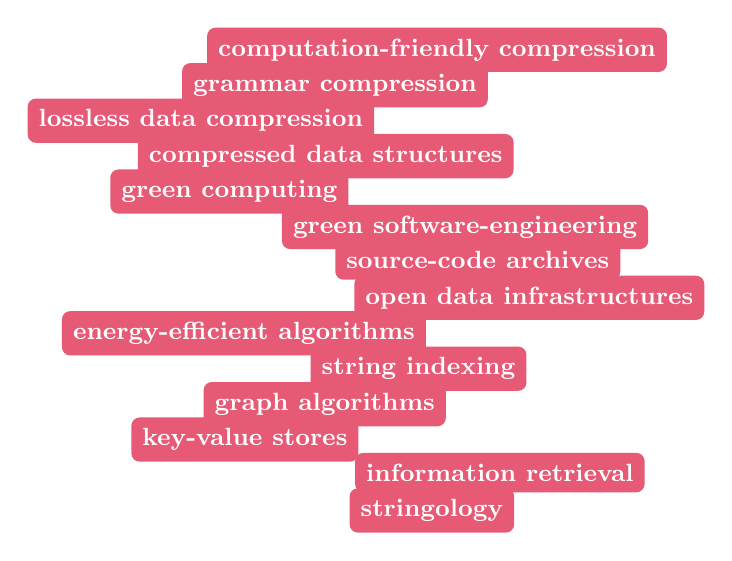
\begin{tikzpicture}
\foreach [count=\i] \skill in {
    computation-friendly compression,
    grammar compression,
    % sparse matrix-vector multiplication,
    lossless data compression,
    compressed data structures,
    green computing,
    green software-engineering,
    source-code archives,
    open data infrastructures,
    energy-efficient algorithms,
    string indexing,
    graph algorithms,
    key-value stores,
    information retrieval,
    stringology
} {
    \node[fill=accent!70!white, rounded corners=3pt, inner sep=4pt, 
          anchor=base, font=\small\bfseries\color{white}] 
        at (rand*2.2, -\i*0.45) {\skill};
}
\end{tikzpicture}
\end{center}
\end{leftcolumn}

% Right Column: Proficiencies (with compatible icons)
\begin{rightcolumn}
\vspace{1em}
\textbf{\textcolor{accent}{\faCode\ Core Tech Stack}} \\
\vspace{.5em}

\begin{tabular}{@{}ll@{}}
\faFileCode \ \textbf{C/C++} & (Expert, C++11/14/17, cmake,\\ & pthread, parallel pattern) \\  % File icon substitute
\faFlask\ \textbf{Python} & (NumPy, pybind11) \\         % Flask for Python
\faTerminal\ \textbf{Bash} & (Scripting/Automation) \\
\faCoffee\ \textbf{Java} & (Prior experience) \\
\faCode\ \textbf{JavaScript} \\
\end{tabular}

\vspace{1em}

\textbf{\textcolor{accent}{\faWrench\ Tools}} \\
\vspace{.5em}
\begin{itemize}[nosep, leftmargin=1em]
    \item \faBug\ CLion (CMake, Debugging)
    \item \faGithub\ VS + Copilot + git
    \item \faDatabase\ RocksDB, Boost
    \item \faServer\ Docker/Compose (Good)
\end{itemize}
\end{rightcolumn}

\end{paracol}
\begin{paracol}{1}

\smallskip

\cvsection{Teaching}

\end{paracol}
\begin{paracol}{1} %\begin{paracol}{2}

\cvevent{Tutor}{``Laboratorio II''}{Sem.~I, A.Y.~23/24}{University of Pisa}

Tutoring (conducted in Italian) for the undergraduate course of ``Laboratorio II'' (24 hours).

\divider %\switchcolumn

\cvevent{Tutor}{``Laboratorio I-A''}{Sem.~I, A.Y.~21/22}{University of Pisa}

Tutoring (conducted in Italian) for the undergraduate course of ``Laboratorio I-A'' (20 hours).

\end{paracol}
\begin{paracol}{1}

\newpage %\smallskip

\cvsection{Natural languages}
I get by with several languages, with varying levels of active engagement and passive comprehension. These include the following.

\divider 

\cvskill{English}{5}
{\em CEFR C1/C2}. Professional proficiency in all communication skills.

% \divider 

\cvskill{Deutsch [German]}{3}
{\em CEFR B1}. Certified language proficiency from the Centre for Applied Linguistics (CLA), UNIPG, Perugia, Italy (July 2017).

% \divider 

\cvskill{Castellano [Spanish]}{3}
{\em CEFR B1-B2}. Strong listening and reading comprehension; experience attending scientific seminars in Spanish; AI-assisted writing.

% \divider 

\cvskill{{\hindi हिन्दी} [Hindi]}{1}
{\em CEFR A2}. Basic grammar and vocabulary knowledge. Gboard-assisted writing; no handwriting.

% \divider 

\cvskill{Italiano [Italian]}{5}
Native speaker fluency.

\smallskip

% \cvsection{Miscellanea}
% \begin{itemize}
%     \item 
%     European Computer Driving Licence (ECDL)
    
%     \item
%     B -- Motor car driving licence
% \end{itemize}

\cvsection{Hobbies \& Community Engagement}

In my spare time, I actively contribute to open-knowledge and collaborative projects. 
As a Wikipedia editor, I have created and improved hundreds of articles and more recently shifted to technical contributions within the Wikimedia ecosystem, particularly on Wikidata and Meta-Wiki. I frequently collaborate with technical contributors from India and other regions, fostering cross-cultural exchanges and advocating for open data as a tool for democratising knowledge access.

\divider 

All of the above statements are true in accordance with the regulations on substitute declarations as per Article 46 et seq. of the Italian Presidential Decree 445/2000.

\medskip

\centering
% Paris, France. 9\textsuperscript{th} July 2025\\
Pisa, Italy. 25\textsuperscript{th} January 2026\\
\smallskip
\includegraphics[width=.3\linewidth]{signature.pdf}


\end{paracol}


\end{document}
